
\section{误差棒}
\label{sec:errorbars}

{
\def\pgfplotserror#1{\ensuremath{\epsilon_{#1}}}

误差棒用于表示一个数据点的可靠程度。通常，一个数据点就是 $(x,y)$。可靠程度由附加的值来表示，也就是通过一个误差界 $\pgfplotserror{x}$ 来刻画绘图数据中给出的坐标 $x$ 与精确值 $\tilde x$（该值未知）之间的差异。可靠程度可以同时针对 $x$ 和 $y$ 独立给出（尽管 $y$ 通常是更典型的对象）。误差界可以表示为\emph{绝对}误差，即形如
%
    \begin{equation*}
        \lvert{x-\tilde x}\rvert \le \pgfplotserror{x}, \quad
        \lvert{y-\tilde y}\rvert \le \pgfplotserror{y}
    \end{equation*}
%
其中 $\tilde x$ 和 $\tilde y$ 是（未知的）精确值，而 $x$ 和 $y$ 是绘图的实际值。不过，误差界也可以相对于输入值给出，即形如
%
    \begin{equation*}
        \frac{\lvert{x-\tilde x}\rvert} {\lvert\tilde x\rvert} \le \pgfplotserror{x},
            \quad
        \frac{\lvert{y-\tilde y}\rvert} {\lvert\tilde y\rvert} \le \pgfplotserror{y}.
    \end{equation*}
%
相对误差为 $10\%$ 时，对应于误差值 $0.1$（相对于精确量 $\tilde y$）。显然，相对误差只有在精确值不为零时才有用，即 $\tilde x, \tilde y \neq 0$。

\PGFPlots{} 允许为每个坐标独立提供“误差值”。因此，它可能找到某个值 $\pgfplotserror{x}$ 和/或 $\pgfplotserror{y}$。根据配置的不同，它会将遇到的值解释为绝对误差或相对误差。误差值可以对每个坐标都相同，例如当你知道每个 $y$ 坐标都有固定的 $10\%$ 误差时。误差值也可以对每个坐标都不同，这时称其为“显式给出”。事实上，\PGFPlots{} 还支持\emph{非对称}误差值，也就是说误差的下界可以与上界不同。因此，一个二维数据点 $(x,y)$ 最多可以有四个不同的误差值，这些都需要由最终用户提供。

因此，最终用户必须提供所有需要的误差值，以及一个配置，用以说明这些值应被解释为相对误差还是绝对误差，以及这些值是应对每个数据点显式给出，还是固定不变。

\begin{codeexample}[]
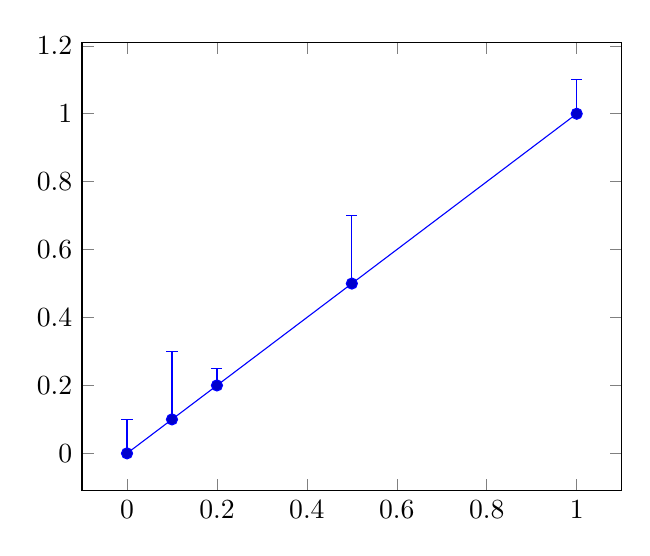
\begin{tikzpicture}
\begin{axis}
    \addplot+ [
        error bars/.cd,
            y dir=plus,y explicit,
    ] coordinates {
        (0,0)     +- (0.5,0.1)
        (0.1,0.1) +- (0.05,0.2)
        (0.2,0.2) +- (0,0.05)
        (0.5,0.5) +- (0.1,0.2)
        (1,1)     +- (0.3,0.1)
    };
\end{axis}
\end{tikzpicture}
\end{codeexample}

前一个例子有两个键：|y dir=plus| 配置 \PGFPlots{} 为 $y$ 坐标\emph{启用}误差棒，但只启用上界。键 |y explicit| 告诉 \PGFPlots{} 在输入数据流中预期为\emph{绝对}值。在上面的例子中，输入数据流是一个 |\addplot coordinates|，它使用特殊的误差值语法 |+- |$(\pgfplotserror{x}, \pgfplotserror{y})$，详见 Section~\ref{sec:errorvalues:coords}。

如果输入数据包含比实际需要更多的误差值，也是允许的：上面的例子同时给出了 $x$ 和 $y$ 的误差值，并且它还包含下界（因为 |+-| 同时定义上界和下界）。

因此，其余的值也可以被可视化：
%
\begin{codeexample}[]
\begin{tikzpicture}
\begin{axis}
    \addplot+ [
        error bars/.cd,
            y dir=both,y explicit,
            x dir=both,x explicit,
    ] coordinates {
        (0,0)     +- (0.5,0.1)
        (0.1,0.1) +- (0.05,0.2)
        (0.2,0.2) +- (0,0.05)
        (0.5,0.5) +- (0.1,0.2)
        (1,1)     +- (0.3,0.1)
    };
\end{axis}
\end{tikzpicture}
\end{codeexample}

误差棒继承相关绘图的所有绘图选项，但它们使用自己的 |error mark| 和附加的样式参数。

\begin{pgfplotsxykey}{error bars/\x\ dir=\mchoice{none,plus,minus,both} (initially none)}
    初始配置 \declareandlabel{none} 在给定方向上完全不绘制误差棒。

    配置 \declareandlabel{plus} 仅在感兴趣的方向上绘制上界。

    配置 \declareandlabel{minus} 仅在感兴趣的方向上绘制下界。

    配置 \declareandlabel{both} 在感兴趣的方向上同时绘制上界和下界。

    在每种情况下，实际的误差值及其性质（绝对或相对）都由其他选项确定（见下文）。如果由于某种原因误差值缺失，则省略该误差棒。
\end{pgfplotsxykey}

\begin{pgfplotsxykey}{error bars/\x\ fixed=\marg{value} (initially 0)}
    为所有输入坐标提供一个公共的绝对误差 $\pgfplotserror x=\text{\meta{value}}$。
    %
\begin{codeexample}[]
\begin{tikzpicture}
\begin{axis}
    \addplot+ [
        error bars/.cd,
            y dir=both,y fixed=0.1,
    ] coordinates {
        (0,0)
        (0.1,0.1)
        (0.2,0.2)
        (0.5,0.5)
        (1,1)
    };
\end{axis}
\end{tikzpicture}
\end{codeexample}

    对于线性 $x$ 坐标轴，误差标记绘制在 $x \pm \pgfplotserror x$ 处；而对于对数 $x$ 坐标轴，则绘制在 $\log( x \pm \pgfplotserror x)$ 处。
\end{pgfplotsxykey}

\begin{pgfplotsxykey}{error bars/\x\ fixed relative=\marg{percent} (initially 0)}
    为所有输入坐标提供一个公共的相对误差 $\pgfplotserror x = \text{\meta{percent}} \cdot x$。因此，参数 \meta{percent} 是相对于输入 $x$ 坐标给出的，即 $\text{\meta{percent}} = 1$ 表示 $100\%$。

    因此，对于线性坐标轴，误差标记放置在 $x \cdot (1 \pm \pgfplotserror x)$ 处；对于对数坐标轴，则放置在 $\log(x \cdot (1 \pm \pgfplotserror x))$ 处。线性坐标轴的计算以浮点数进行，对数刻度则利用恒等式 $\log(x \cdot (1 \pm \pgfplotserror x)) = \log(x) + \log( 1 \pm \pgfplotserror x)$ 进行。

    下面的例子表明，固定误差值 $\pgfplotserror{x}$ 与输入值无关。
    %
\begin{codeexample}[]
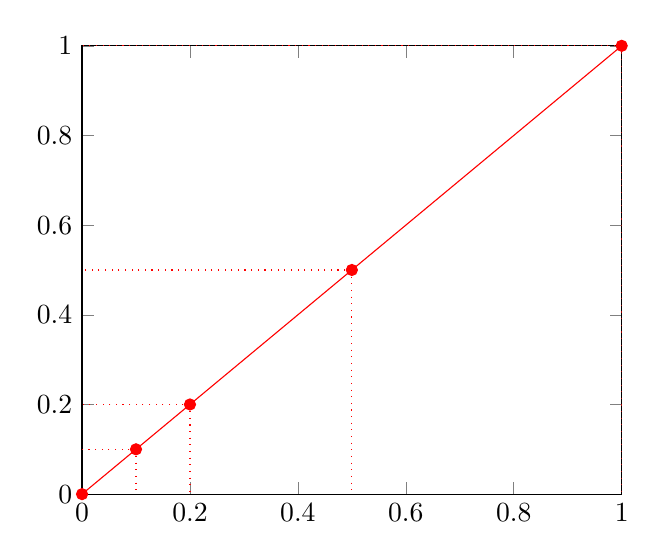
\begin{tikzpicture}
\begin{axis}[enlargelimits=false]
    \addplot [red,mark=*] plot [
        error bars/.cd,
            y dir=minus,y fixed relative=1,
            x dir=minus,x fixed relative=1,
            error mark=none,
            error bar style={dotted},
    ] coordinates {
        (0,0) (0.1,0.1) (0.2,0.2)
        (0.5,0.5) (1,1)
    };
\end{axis}
\end{tikzpicture}
\end{codeexample}
\end{pgfplotsxykey}

\begin{pgfplotsxykey}{error bars/\x\ explicit}
    配置误差棒算法，在任何存在用户指定误差的输入坐标处绘制 $x$ 误差棒。每个误差被解释为绝对误差，详见 |x fixed|。

    误差的不同输入格式在 Section~\ref{sec:errorbar:input} 中描述。
\end{pgfplotsxykey}

\begin{pgfplotsxykey}{error bars/\x\ explicit relative}
    配置误差棒算法，在任何存在用户指定误差的输入坐标处绘制 $x$ 误差棒。每个误差被解释为相对误差，也就是说误差标记放置在 $x (1 \pm \text{\meta{value}}(x))$ 处（其工作方式与 |error bars/x fixed relative| 相同）。
    %
\begin{codeexample}[]
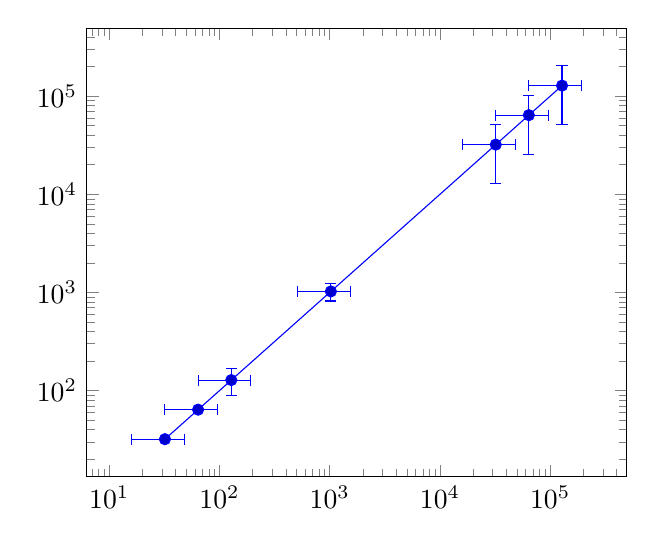
\begin{tikzpicture}
\begin{loglogaxis}
    \addplot+ [
        error bars/.cd,
            x dir=both,x fixed relative=0.5,
            y dir=both,y explicit relative,
    ] table [x=x,y=y,y error=error] {
        x       y       error
        32      32      0
        64      64      0
        128     128     0.3
        1024    1024    0.2
        32068   32068   0.6
        64000   64000   0.6
        128000  128000  0.6
    };
\end{loglogaxis}
\end{tikzpicture}
\end{codeexample}
\end{pgfplotsxykey}

\begin{pgfplotskey}{error bars/error mark=\meta{marker} (initially -)}
    为任何误差棒设置一个误差标记。\meta{marker} 应当是一个有效的绘图标记，参见 Section~\ref{sec:markers}。
    %
\begin{codeexample}[]
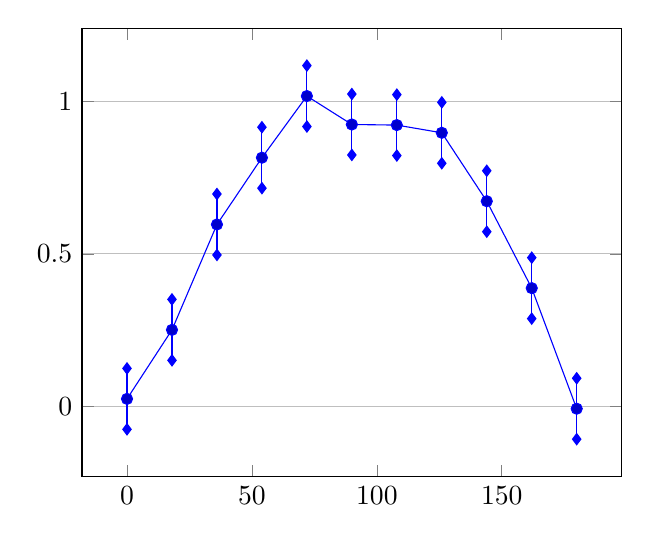
\begin{tikzpicture}
    \pgfmathsetseed{42}
\begin{axis}[
    ymajorgrids,
]
    \addplot+ [
        domain=0:180,
        samples=11,
        error bars/.cd,
            y dir=both, y fixed=0.1,
            error mark=diamond*,
    ] {sin(x) + rand*0.1};
\end{axis}
\end{tikzpicture}
\end{codeexample}
\end{pgfplotskey}

\begin{pgfplotskey}{error bars/error mark options=\marg{key-value-list} (initially rotate=90)}
    为任何误差标记设置一个键值选项列表。此选项的工作方式与 \Tikz{} 的 `|mark options|' 键类似。
\end{pgfplotskey}

\begin{pgfplotskey}{error bars/error bar style=\marg{key-value-list}}
    将参数追加到 `|/pgfplots/every error bar|'，后者在每个误差棒的开头被安装。
\end{pgfplotskey}

\begin{pgfplotscodetwokey}{error bars/draw error bar}
    允许更改误差棒的默认绘图命令。这两个参数是
    %
    \begin{itemize}
        \item 源点，$(x,y)$，以及
        \item 目标点，$(\tilde x,\tilde y)$。
    \end{itemize}
    %
    两者都由 \PGFPlots{} 根据上述选项确定。默认代码为
    %
\begin{codeexample}[code only]
\pgfplotsset{
    /pgfplots/error bars/draw error bar/.code 2 args={
        \pgfkeysgetvalue{/pgfplots/error bars/error mark}
            {\pgfplotserrorbarsmark}
        \pgfkeysgetvalue{/pgfplots/error bars/error mark options}
            {\pgfplotserrorbarsmarkopts}
        \draw #1 -- #2 node [pos=1,sloped,allow upside down] {
            \expandafter\tikz\expandafter[\pgfplotserrorbarsmarkopts]{
                \expandafter\pgfuseplotmark\expandafter{\pgfplotserrorbarsmark}
                \pgfusepath{stroke}}
        };
    },
}
\end{codeexample}
\end{pgfplotscodetwokey}


\subsection{误差坐标的输入格式}
\label{sec:errorbar:input}

为单个数据点提供显式误差估计的误差棒需要某种输入格式。这适用于 |error bars/x explicit| 和 |error bars/x explicit relative|。


\subsubsection{误差坐标与坐标列表}
\label{sec:errorvalues:coords}

误差棒坐标可以从 `|\addplot coordinates|' 中读取，在其中它们按如下方式跟在数据点之后给出：
%
\begin{codeexample}[code only]
\addplot coordinates {
    (1,2) +- (0.4,0.2)
    (2,4) +- (1,0)
    (3,5)
    (4,6) +- (0.3,0.001)
}
\end{codeexample}
%
其中 $(1,2) \pm (0.4,0.2)$ 是第一个坐标，$(2,4) \pm (1,0)$ 是第二个，依此类推。点 $(3,5)$ 没有误差坐标。语法 \declareandlabel{+-} 定义\emph{对称}误差值，也就是说上界和下界取相同的值。

或者，也可以使用 \declareandlabel{-=} 和 \declareandlabel{+=} 之一来定义非对称值：
%
\begin{codeexample}[]
\begin{tikzpicture}
\begin{axis}
    \addplot+ [
        error bars/.cd,
            x dir=both, x explicit,
            y dir=both, y explicit,
    ] coordinates {
        (1.1,0.9) += (0.4,0.2) -= (0.1,0.1)
        (2.7,2)   -= (1,0)
        (3,3)
        (3.8,4.2) +- (0.3,0.2)
    };
\end{axis}
\end{tikzpicture}
\end{codeexample}
%
如果为同一个坐标指定了多个项（例如多个 |+=|），则以最后一个为准。

请记住，这些误差值只有在 |x dir| 和 |y dir| 被适当设置时，才会作为误差棒显示出来。

输入类型 |\addplot coordinates| 还允许 |point meta=explicit|，即形如
%
\begin{codeexample}[code only]
\addplot coordinates {(0,0) [4]};
\end{codeexample}
%
这可以与误差值结合使用。不过，方括号中的 point meta 值必须是最后一项：
%
\begin{codeexample}[code only]
\addplot coordinates {(0,0) +- (0.1,0.2) [4]};
\end{codeexample}


\subsubsection{误差坐标与表格输入}

`|\addplot table|' 的格式为

\begin{pgfplotsxykeylist}{%
    table/\x\ error=\marg{column name},
    table/\x\ error index=\marg{column index},
    table/\x\ error expr=\marg{math expression}%
}
    这些键定义了带显式误差值的误差棒的输入来源。

    |x error| 方法提供一个输入列名（或别名），\todosp{我认为下面例子前后的两段文字几乎是一样的} |x error index| 方法提供输入列\emph{索引}，而 |x error expr| 的工作方式与 |table/x expr| 相同：它允许任意的数学表达式，这些表达式可以使用 |\thisrow|\marg{col name} 依赖于任意数量的表格列。
    %
\begin{codeexample}[]
\begin{tikzpicture}
\begin{axis}
    \addplot+ [
        error bars/.cd,
            x dir=both, x explicit,
            y dir=both, y explicit,
    ] table [y error=error] {
        x   y   error
        1   0.9 0.4
        2   2.1 0.2
        3   3   0.1
        4   4.2 0.3
    };
\end{axis}
\end{tikzpicture}
\end{codeexample}

    此外，还可以使用以下方式提供列\emph{索引}：
    %
\begin{codeexample}[code only]
\addplot table[x error index=COLINDEX,y error index=COLINDEX]
\end{codeexample}
    %
    这些选项的使用方式与 `|x|' 和 `|x index|' 选项相同。

    如果你需要指定数学表达式，可以使用 |x error expr|：
    %
\begin{codeexample}[code only]
\addplot table[x error expr=\thisrow{errorx}^2]
\end{codeexample}
    %
    这与 |x expr| 类似。
    %
\end{pgfplotsxykeylist}

\begin{pgfplotsxykeylist}{%
    table/\x\ error plus=\marg{column name},
    table/\x\ error plus index=\marg{column index},
    table/\x\ error plus expr=\marg{math expression},
    table/\x\ error minus=\marg{column name},
    table/\x\ error minus index=\marg{column index},
    table/\x\ error minus expr=\marg{math expression}%
}
    这些键定义了带\emph{非对称}误差值的误差棒的输入来源，也就是说上界和下界取不同的值。

    它们的使用方式与 |x error| 相同。事实上，|x error| 只是一个将 |x error plus| 和 |x error minus| 都设置为相同值的样式。
    %
\begin{codeexample}[]
\begin{tikzpicture}
\begin{axis}
    \addplot+ [
        error bars/.cd,
            x dir=both, x explicit,
            y dir=both, y explicit,
    ] table [
        x error plus=ex+,
        x error minus=ex-,
        y error plus=ey+,
        y error minus=ey-,
    ] {
        x   y   ex+  ey+  ex-  ey-
        1.1 0.9 0.4  0.2  0.1  0.1
        2.7 2   0    0    1    0
        3   3   0    0    0    0
        3.8 4.2 0.3  0.2  0.3  0.2
    };
\end{axis}
\end{tikzpicture}
\end{codeexample}
\end{pgfplotsxykeylist}

}
